\documentclass[a4paper,12pt]{article}
\usepackage[utf8]{inputenc}
\usepackage{hyperref}
\usepackage{graphicx}
\usepackage{float}
\graphicspath{ {images/} }

\begin{document}

\begin{titlepage}

\newcommand{\HRule}{\rule{\linewidth}{0.5mm}} % Defines a new command for the horizontal lines, change thickness here

\center % Center everything on the page
 
%----------------------------------------------------------------------------------------
%-	HEADING SECTIONS
%----------------------------------------------------------------------------------------

\textsc{\LARGE University of Pretoria}\\[1.5cm]
\textsc{\Large COS 301 - Software Engineering}\\[0.5cm]
\textsc{\large The Savage Ru's}\\[0.5cm]

%----------------------------------------------------------------------------------------
%-	TITLE SECTION
%----------------------------------------------------------------------------------------

\HRule \\[0.4cm]
{ \huge \bfseries User Manual}\\ % Title of your document
\HRule \\[1.5cm]
 
%----------------------------------------------------------------------------------------
%-	AUTHOR SECTION
%----------------------------------------------------------------------------------------

\begin{minipage}{0.4\textwidth}
\begin{flushleft} \large
\emph{Author(s):}\\
Jodan \textsc{Alberts}\\ % Your name
Mark \textsc{Klingenberg}\\
Una \textsc{Rambani}\\
Ruan \textsc{Klinkert}\\
\end{flushleft}
\end{minipage}
~
\begin{minipage}{0.4\textwidth}
\begin{flushright} \large
\emph{Student number(s):} \\
14395283\\ % Student number
14020272\\
14004489\\
14022282\\

\end{flushright}

\end{minipage}\\[0.5cm]


%----------------------------------------------------------------------------------------
%-	DATE SECTION
%----------------------------------------------------------------------------------------

\centering
	
\includegraphics[width=80mm]{SavageRu.jpg}

{\large \today}\\[3cm] % Date, change the \today to a set date if you want to be precise

\centering
	\textsc{\LARGE Epi-Use labs project}\\[0.5cm]
	\textsc{\Large VizARD}\\[0.5cm]
	\textsc{\Large User Manual version 0.1}\\[0.5cm]
	
\includegraphics[width=\textwidth]{images/vizard.jpg}
%----------------------------------------------------------------------------------------

\vfill % Fill the rest of the page with whitespace

\end{titlepage}

\newpage

\tableofcontents

\newpage

\section{Introduction}

This is the user manual for the vizARD Augmented Reality application being developed for EPI-USE Labs by The Savage Ru's.

VizARD is a mobile application which will allow a user to take a picture of tabulated data and then view, automatically generated, 3D graphs of the data projected onto the document of which the image was taken.


\section{Vision}
EPI-USE Labs (henceforth referred to as "the client") intends for the VizARD application to be used by a large variety of mobile device users across both Android and iOS platforms. VizARD helps to simplify the analysis of numerical data through visualization, in the form of automatically generated 3D graphs.

Fundamentally, the system will allow a user to take a picture of a table of numerical data which he/she may need to interpret. The application will then use OCR (Optical Character Recognition) to read the data from the picture. It will then decide on an appropriate graph for the type of data and generate a graph for the data. After the graph is generated, it will project a 3D model of the graph onto the image (or, ideally, onto a live stream of the paper) for the user to view.

Additionally, the system will allow users to send images (or screen captures) of generated graphs to other devices via popular social media channels.

Typically usage will be as follows:
\begin{itemize}
	\item The user (possibly a businessman) finds tabular data he/she would like to analyse more easily.
	\item The user opens the app.
	\item Once the app is open and loaded, the user takes a picture of the table he/she would like to analyse.
	\item The user receives a notification that the graph has been generated and the generated graph is displayed on the screen (mapped onto the paper).
	\item The user taps on the "Share" button and is presented with several options through which he/she can share the graph.
	\item An option is selected and an image of the graph is sent to the other user.
\end{itemize}

\newpage
\section{Background}

It is much simpler for us to recognize patterns and make quick analysis of data if it is presented to us in visual form. A simple example for the use of such an application would be a principal at a school who is presented with the Mathematics results of a particular grade for several quarters, such an application would make it very simple for him to quickly visualize the numeric data and see the trend.
\newline
\newline
The problem at hand is that there is a lot of information to go around and so little time to process. In a society that demands us to make decisions quickly, it would be wise to have a tool that aids the decision making process by making the information easier to digest and that is what vizARD intends to do.
\newline
\newline
Potential users could range from students, researchers, people in business, managers at stores and anyone else who would like to visualize data on the go.
		

\newpage

%%--------------------------------------INSTALLATION  ----------------------------------------
\section{Installation}
To access the VizARD application one must first install it, currently this is done by getting the vizARD apk file, and installing it onto your android mobile phone (allow for the installation from unknown sources). In the future this app will be available through the Google play store.

%%-------------------------------------GETTING STARTED ----------------------------------------
\section{Getting Started}
Once the app has been installed the user simply need to click on the application named VizARD, this will bring the user into a launching screen shown in figure 1.\\
\begin{figure}[H]
\centering
	
\includegraphics[width=50mm]{images/launch.png}
	\caption{launching screen \label{overflow}}
\end{figure}

Once the app has finished launching the user will be greated by the landing screen.
%%-------------------------------------LANDING SCREEN ----------------------------------------
\section{Landing Screen}
Once the app has completed loading it will then bring you to a screen that looks like figure 2, this screen shows what the camera is looking at as well as having two buttons currently, these are the capture data circle (Figure 3) that should be familiar to users of snapchat, as well as the View Previous graphs button (figure 4).

\begin{figure}[H]
\centering
	\includegraphics[width=50mm]{images/landing.png}
	\caption{landing screen \label{overflow}}
\end{figure}

\begin{figure}[H]
  \centering
  \begin{minipage}[b]{0.4\textwidth}
    
\includegraphics[width=50mm]{images/capture.png}
    \caption{Capture icon.}
  \end{minipage}
  \hfill
  \begin{minipage}[b]{0.4\textwidth}
    
\includegraphics[width=50mm]{images/graphRed.png}
    \caption{View Graphs.}
  \end{minipage}
\end{figure}



%%----------------------------------ON CAPTURE CLICK-----------------------------------------
\subsection{On Capture Circle click}
When a user clicks the capture data circle (figure 3) it will chose the table that is being viewed as the target for the 3D graph that will be generated, it will also send the image to a server to allow for optical character recognition of the data to make the graph, while this is occuring we plan to have some loading model to be placed on the target while the user waits. Once it has generated the graph the app moves to the display screen.

%%----------------------------DISPLAY GRAPH CLICK------------------------------------------------
\subsection{On View graphs click}
When a user clicks the View Graphs button (figure 4) currently nothing will happen as this section has not been implemented but we plan on it taking the user to screen shots of previous graphs they have decided to save. 
\newpage
%%----------------------------DISPLAY SCREEN------------------------------------------------
\section{Dispay Screen}
Once the app has completed generating the graph it will then bring you to a display screen that looks like figure 5, this screen shows the newly generated graph that has been mapped onto the target two buttons currently, these are the share graph button (Figure 6), as well as the edit graphs button (figure 6). We plan on implementing a save graph button that will also be here and will take a screen shot of the graph and save it. 

\begin{figure}[H]
\centering
	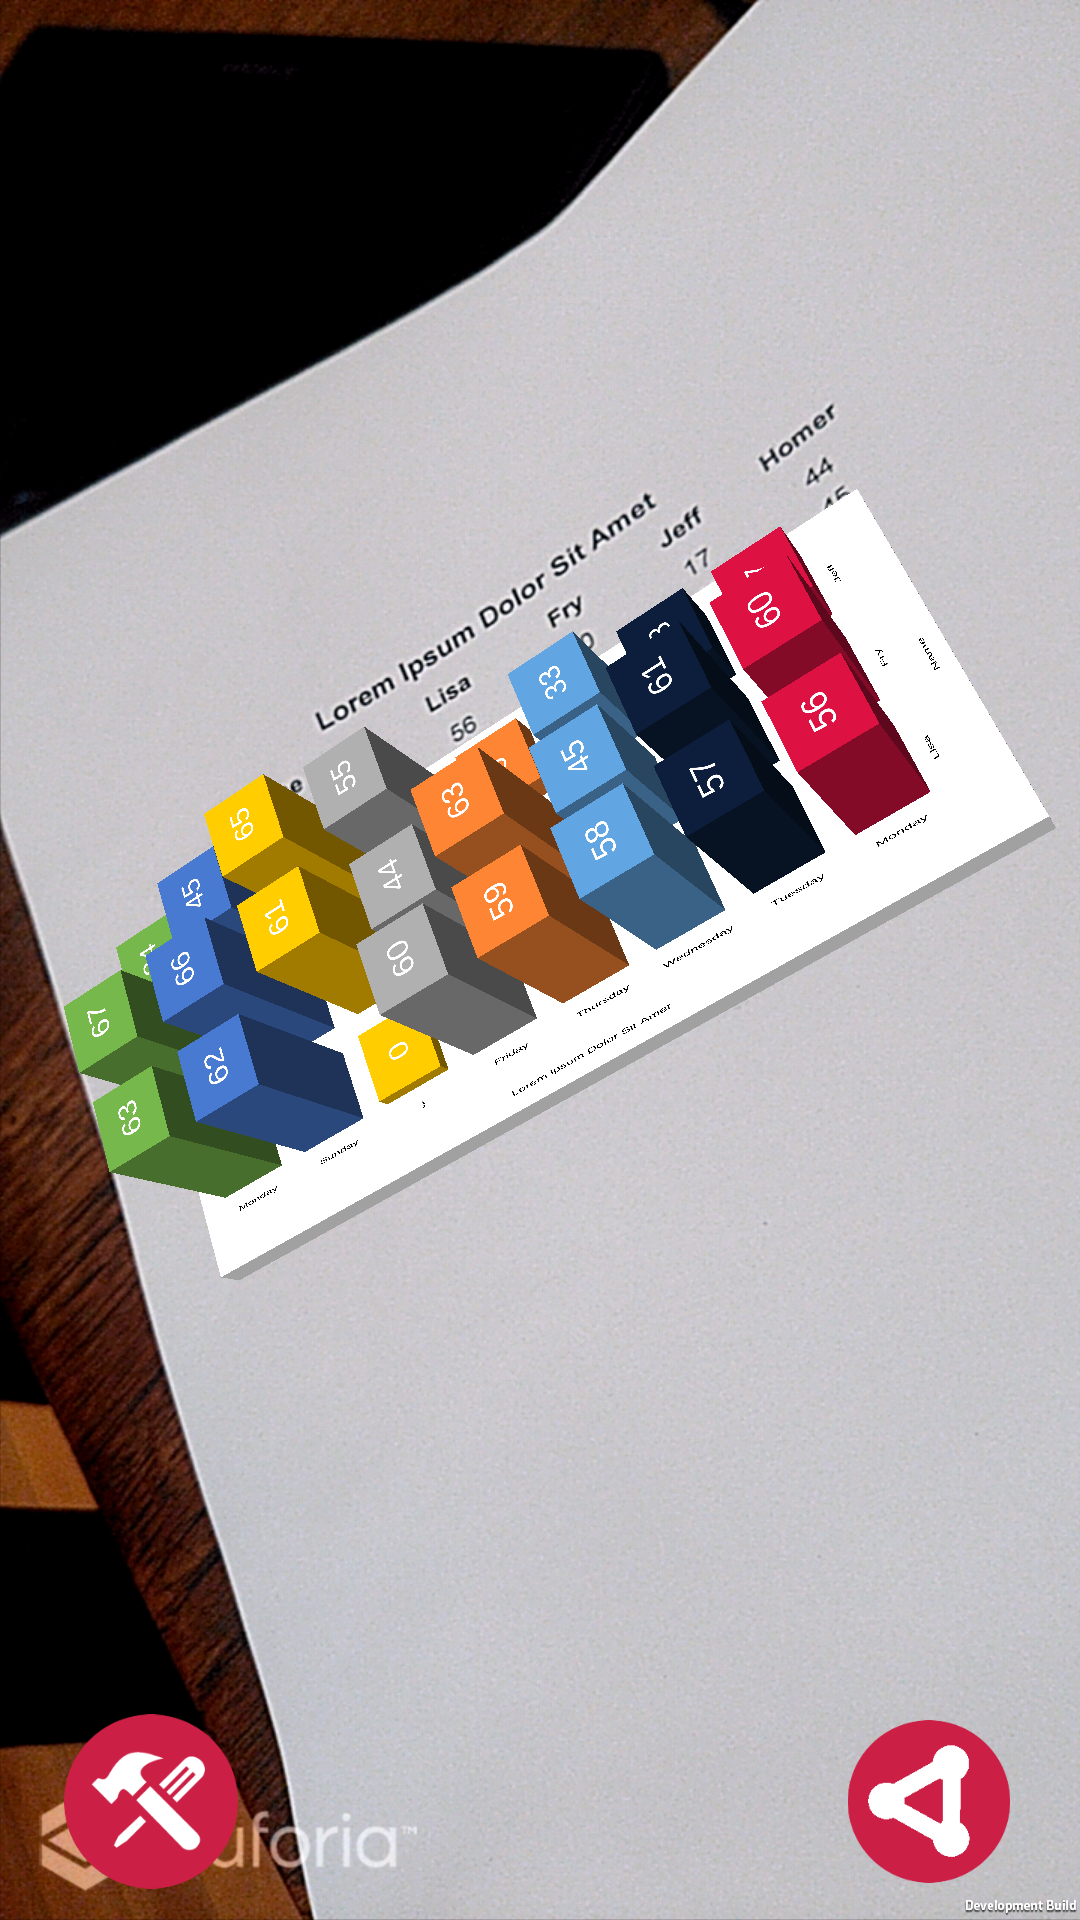
\includegraphics[width=\textwidth]{images/graph.png}
	\caption{display screen \label{overflow}}
\end{figure}

\begin{figure}[H]
  \centering
  \begin{minipage}[b]{0.4\textwidth}
    
\includegraphics[width=50mm]{images/editRed.png}
    \caption{Edit button}
  \end{minipage}
  \hfill
  \begin{minipage}[b]{0.4\textwidth}
    
\includegraphics[width=50mm]{images/shareRed.png}
    \caption{Share button}
  \end{minipage}
\end{figure}
\newpage
%------------------------on edit click------------------------------------
\subsection{On Edit Button click}
The edit button has not yet been implemented but once it has when a user clicks it, it will allow for the user to change the style of graph (bar to pie, pie to line, etc...), switch graph axis (switch the data on the x axis with the data on the y axis) and possibly to change the data that has been used to draw the graph. 

%------------------------on Share click------------------------------------

\subsection{On Share Button Click}
The share button has also yet to be implemented but once it has when a user clicks it the app will take a screen capture of the graph and open up genral sharing option such as share to facebook or whatsapp.

\subsection{Improvements}
For the display screen we are contemplating having a hamburger menu that hides these two buttons until clicked so that they take up less screen real estate from the graph.

\end{document}
